\chapter{Setup of data and project}
In this chapter we will discuss the setup of the project. The first step was to read in the teff genomic data in R in a way it can be processed by the seqinr package and be converted to work as a string sequences as required for compability with Darwin processes. The next step was to read in tRNA gene count for different genomes to estimate the tRNA availability in different genomes and to decide on the optimality of the codons used. To conclude the setup phase we implemented a graphical representation over genes to show a moving average of where in the gene optimal codons are used based on the fraction of codon tRNA gene counts to the maximal count for the amino acid to be translated. 

\section{Getting familiar with the data}
Before the project was set-up the initial task was to gather information for calculating one of the first defined and most basic codon bias index called \hyperlink{function:Fop}{frequency of optimal codons (Fop)}. The optimality of a codon can be estimated by the usage in the given gene, the transcriptome or by accessing the numbers of tRNA genes found in the genome. As we have already the \hyperlink{data:tRNAlist}{data of tRNA genes for the teff genome} available, this was the choice to work with and to import the information for closely related species for mays and millet.

\subsection{tRNA gene statistics and optimality of codons}
First we addressed a public database containing the tRNA gene counts, after detecting them by tRNAscan and filtering the non-confident hits. Later tRNA gene numbers for all available eukariotic, bacterial, archaea and one viral genome was extracted from tRNAscan-SE v.1.3 run statistics of the GtRNAdb 2.0 (available at
\href{http://gtrnadb.ucsc.edu/GtRNAdb2/genomes/}{Genomic tRNA Database 2.0}, http://gtrnadb.ucsc.edu/GtRNAdb2/genomes/). \cite{Chan2016} %[Chan PP et al. 2016]
The first script for extracting the numbers was:
  \lstinputlisting[language=R, breaklines=true]{codes/readstats.R}
The statistic file from a html page for mays is given below as demonstration: 
  \lstinputlisting[language=HTML, breaklines=true]{codes/Zmays.stats}    
 
However \hyperlink{function:readintronic}{this code} had to be adapted because it is only reading in the tRNA genes with introns. Therefore, \hyperlink{function:readstats}{another function} was implemented to read in the total tRNA gene count. Interestingly, by browsing some of the output data from tRNAscan for other species we discovered some that have a huge amount of the alternative usage of the opal stop codon "UGA" that is messing up with the display of the overview in a hierarchical plot for all the tRNA numbers even when standardized for each tRNA, we can see that some of the species show a much higher total number of tRNAs. 

However, there is some inconsistency in the data base in order that a few of the genomes contain so many tRNA genes, that these are overcrowding the graphical representation in a heat map for example (see fig. ~\ref{fig:byrow}).

\begin{figure}[tb] 
\centering 
\includegraphics[width=0.9\columnwidth]{byrow} 
\caption[Heat map for tRNA counts]{Heat map of tRNA gene counts normalized per row in \hyperlink{data:veab}{all species}}
\label{fig:byrow} 
\end{figure}

If we plot the log values of the tRNA gene count and normalize by species (column) then we can see that some species have very low numbers of certain codons that is usually compensated by using another block of codons that are rare in the other kingdoms  (see fig. ~\ref{fig:bycol}). We also observe some species that have a high number of tRNAs where the isoaccepter remains unknown (codon 65). \\

\begin{figure}[tb] 
\centering 
\includegraphics[width=0.9\columnwidth]{logallfa_col} 
\caption[Heat map for log(tRNA counts)]{Heat map of logged(tRNA gene counts) normalized per column in \hyperlink{data:veab}{all species}}
\label{fig:bycol} 
\end{figure}

We can observe that those run statistics, from vertebrates especially non-primate mammals, are littered with tRNA-derived repetitive elements with primary sequences very similar to real tRNAs. So they apply a non-unveiled post filter after the tRNAscan-SE on those genomes before depositing the predictions to GtRNAdb. Therefore, these had to be rebuild from scanning the headers of the fasta files by implementing yet \hyperlink{function:readfasta}{an alternative funtion}, that seems to be consistent with the new version of tRNAscan 2.0 and gave the best results. For that purpose the fasta file name had to be scanned in the index.html file and the fasta files were renamed according to the directory name to facilitate automation. This needed \hyperlink{function:searchfafile}{a helper function} to find those fasta files on the GtRNAdb2 server. One issue was that genomes with names containing \# or \* have to be treated as special cases, as even the browser fails to fetch the files. Therefore \# was replaced with \%23. \\

To read in the output file of tRNAscan for tef, a function \hyperlink{function:rtRNAo}{readtRNAout} was created that converts this file to a table resembling the ones created from GtRNAdb2. \\

In contrast to other codon usage software, the statistics is now enhanced by an 65th line containing undefined aminoacid all other anticodons with degenerated base information are counted to the undefined species as they do in the summary page. \\ 

\section{First functions and analyses}
The project had now the first lines of code that were producing something interesting, however the project should be based on three pillars, namely the code itself, the testing functions and the documentation, including demonstration scripts. Therefore, the R package \textit{statanacoseq} was initiated and the code that produced the first indices and graphical representation rewritten to work as standalone package as well as handling local files. Before we introduce the setup of the package we show some results from the first analyses of the sample data.

\subsection{Optimality of used codons}
The first index to be implemented was the frequency of optimal codons. When the decision on which codons are optimal is made, the calculation of this index is quite basic. The decision can be made by taking the codon usage of the gene alone or the full genome or what we intended to implement first was to make the decision on the availability of tRNAs estimated from the number of tRNA genes that we find in the genome of \textit{E. tef}. For generalization of the function we scanned available information on tRNA gene counts from a public database. However, the retrieved tRNA database turned out to make some problems as discussed above. In conclusion, some of the species had a much higher number of tRNA genes, so that a normalization was necessary to get an overview on the used codons. \\

To decide on optimal codons the number of genes for the given anticodon was divided by the maximal number of genes for a anticodon for the same amino-acid to give fraction to the optimal codon. The codon was accepted as optimal if this fraction was 1. In a list for every genome with available run statistic data, a frame with amino-acid, codon, number of genes, fraction to optimal codon, fraction to all codons, and the decision if it is a optimal codon was stored for the four superkingdoms seperately. To get an overview of the optimality of the codon used in a gene the function \hyperlink{function:plotOCU}{plotOCU} was implemented to show a moving average on the used codon optimality (see fig. ~\ref{fig:plotGC}). \\

\begin{figure}[tb] 
\centering 
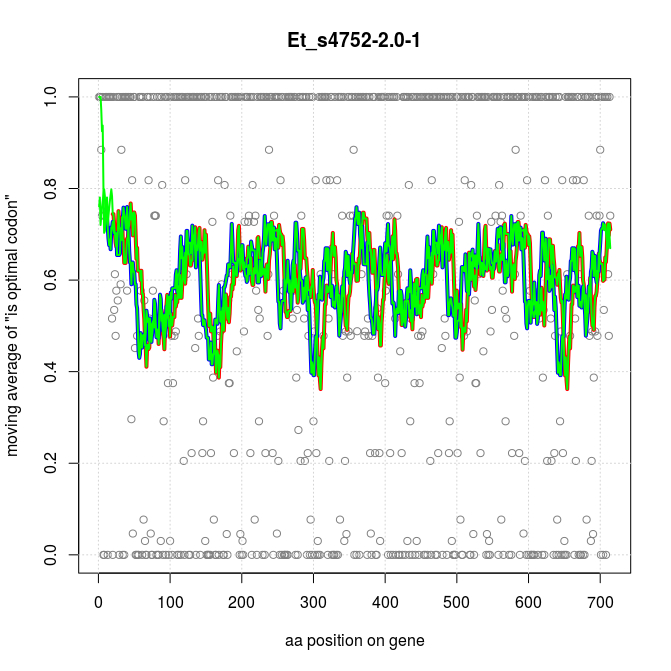
\includegraphics[width=0.9\columnwidth]{fig1_plotOCU} 
\caption[A sample figure from demo plotOCU]{A sample figure (from plot OCU \emph{demo(plotOCU)}, of statanacoseq, got from \url{https://github.com/fredysiegrist/statanacoseq}) shwoing the optimality score of each codon used for coding Similar to Eukaryotic peptide chain release factor subunit 1-3 (eRF1-3) gene of teff.}
\label{fig:plotOCU} 
\end{figure}

One of the expected attributes of the moving average line for the optimality of the used codons is the so called codon ramp \cite{Tuller2010}. The codon ramp describes the phenomenom that rare codons are used at the start of genes. This hypothesis first mainly was proposed for genes with strong translation, but then it has been shown that rare codons at the N terminus increased expression in a general manner. However, when we analyzed some genes from teff, we couldn't observe a overrepresentation of rare codons at the start of the protein translation.  When analysing the moving average of the optionality factor of the codons for the tRNA genes, we don't really detect a codon ramp at the 5' terminus, but the first codon was always optimal. No wonder because there is only one codon for methionine, the start codon. Therefore we should only analyse the aminoacids that have a choice of anti-codons to use. However, the refinement of this code needs still to be implemented.  
Other issues during codon usage analysis was found in the data files of tef that is labeled as validated protein-transcript fasta files: 
first one of the proteins (
Et\_s4372-0.17-1
) was truncated and didn't startet with methionine and was not corresponding to the truncated transcript, secondly the number of transcripts matched the number of proteins, but there was one orphan entry on each side (
Et\_s2692-0.26-1, Et\_s14755-0.7-1
), that had to be filled up with the corresponding entry of the other datafile. 
The files were then corrected and stored as a local copy, however this lead to the condensation of those huge fasta files to a sample data-set incorporated in the package itself that could be used further for demonstration of the functions without running in further issues.

\subsection{GC content at codon sites}
Another basic statistic that can be applied without looking at the full genome is the GC content at the different positions of the codons. If we print the mean GC content of the first two bases against the one at the third codon position for the sample sequences of tef, we can observed that they tend to follow each other there (see fig. ~\ref{fig:plotGC}). This function was implemented at last but shows exemplarly how basic analyses on custom genomes can be implemented in simple codes for comparision these genomic information.

\begin{figure}[tb] 
\centering 
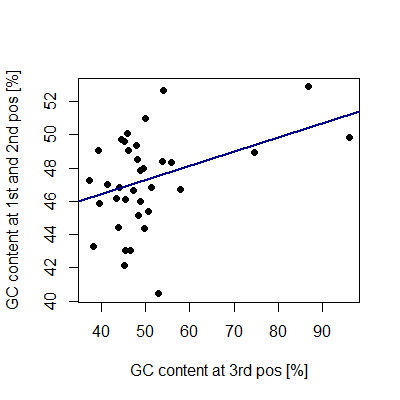
\includegraphics[width=0.5\columnwidth]{plotGC} 
\caption[GC percentage at synonymous sites]{Mean GC content at first and second compared to third site of codon trinucleotide for sample sequences from \hyperlink{function:mylist}{mylist}}
\label{fig:plotGC} 
\end{figure} 


